\documentclass[10pt]{article}

\usepackage{caption}
\usepackage{subcaption}
\usepackage{graphicx}
\usepackage{multirow}
\usepackage{enumerate}

\begin{document}

\section{Exercise 1}

% Gradient descent is an iterative procedure to find the local minimum of a function $f(x)$ by successively looking at values of the function proportional to the direction of the gradient of the function. The iteration stops when the result from two successive steps yields a difference below a specified threshold. This means that once the local minimum is reached, movement along the gradient of a given function will not yield significantly different results. For a scalar function with vector argument inputs, this procedure can be written mathematically as: 
% $$x_{n + 1} = x_n - \eta*\nabla f(x_n).$$

% A start value $x_0$ and a step size $\eta$ is given to start the procedure, as well as a threshold $\beta$. When $|x_{n + 1} - x_n| < \beta$, the procedure stops. It is possible to define different step sizes $\eta$ for each iteration of the gradient descent procedure, but this analysis assumes a constant step size. 

% Testing this gradient descent optimizer on an upside-down Gaussian function with mean $6$ and variance $4$, we expect the minimum to occur at $(6, -1)$, since there is one global minimum. If the function and gradient are defined as: 
% $$f(x) = -e^{\frac{(x - 6)^2}{8}} \qquad \nabla f = \frac{x - 6}{4} e^{\frac{(x - 6)^2}{8}}$$
% (see Figure \ref{fig:gaus}), then the gradient descent algorithm always converges to the correct global minimum. For functions with one minimum, the larger the step value, the faster the algorithm will converge, regardless of how far the initial guess is from the minimum. The threshold dictates how close the numerical solution is from the analytical solution (see Figure \ref{tbl:gaus}).

% \begin{figure}[!ht]
% 	\centering
% 	\makebox[\linewidth][c]{%}
% 	\begin{subfigure}[h]{0.55\textwidth}
% 	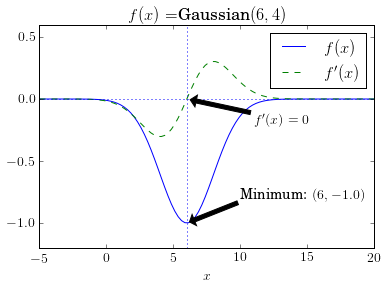
\includegraphics[width=\textwidth]{exercise1a.png}
% 	\caption{Graph of $f(x)$ and its gradient}
% 	\label{fig:gaus}
% 	\end{subfigure}
% 	\begin{subtable}[h]{0.55\textwidth}
% 	\centering
% 	\vspace{12mm}
% 	\begin{tabular}[h]{cccc}
% 		Guess & Step & Iterations & Minimum \\\hline
% 		5 & 0.5 & 21 & (5.934, -.999) \\\hline
% 		5 & 1 & 13 & (5.974, -1.000)  \\\hline
% 		2 & 0.5 & 47 & (5.938, -1.000) \\\hline
% 		2 & 5 & 4 & (5.998, -1.000) \\\hline
% 	\end{tabular}
% 	\vspace{12mm}
% 	\caption{Parameters and results of gradient descent. The threshold was always $0.01$}
% 	\label{tbl:gaus}
% 	\end{subtable}
% 	}\\
% 	\caption{Results for $f(x) = $-Gaussian$(6, 4)$}
% \end{figure}

% The same algorithm can be applied to scalar functions with vector inputs. For example, 
% $$ f(x, y) = (x + 2)^2 + y^2 \qquad \nabla f = 2(x + 2) + 2y$$
% And has one global minimum. In choosing parameters, the smaller the step size and the smaller the threshold, the more iterations are required for the algorithm to converge.

% \begin{figure}[!ht]
% 	\centering
% 	\makebox[\linewidth][c]{%}min}
% 	\begin{subfigure}[b]{0.55\textwidth}
% 		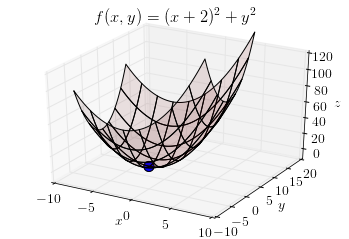
\includegraphics[width=\textwidth]{exercise1c.png}
% 		\caption{$f(x, y)$, $\nabla f$, and the estimated minimum}
% 		\label{fig:nomin}
% 	\end{subfigure}
% 	\begin{subtable}[b]{0.55\textwidth}
% 	\centering
% 	\begin{tabular}[b]{ccccc}
% 		Guess & Step & Thresh & Iterations \\\hline
% 		(0, 0) & 0.5 & 0.01 & 2 \\\hline
% 		(5, 5) & 0.5 & 0.01 & 2  \\\hline
% 		(5, 5) & 0.1 & 0.01 & 25 \\\hline
% 		(5, 5) & 0.1 & 0.001 & 35 \\\hline
% 	\end{tabular}
% 	\vspace{10mm}
% 	\caption{Parameters and results of gradient descent. The minimum always came out to be $(-2, 0, 0)$}
% 	\label{tbl:nomin}
% 	\end{subtable}
% 	}\\
% 	\caption{Using gradient descent to estimate the minimum of a scalar function with vector inputs}
% \end{figure}

% For functions without a global minimum (non-convex functions), the choice of input parameters dictates not only how fast the algorithm converges, but also the value at which it converges. For example, the function
% $$f(x) = \sin(x + \frac{\pi}{2}) + 3 \qquad \nabla f = \cos(x + \frac{\pi}{2})$$
% has local minima at $(2(n + 1)\pi, 2)$ for all $n$ (see Figure \ref{fig:nomin}). When the initial guess for gradient descent is chosen to be closer to the local minima at $-\pi$, the algorithm estimates that to be the local minimum, and vice versa for $\pi$. If the initial guess is given at $0$, which is a local maximum, the algorithm does not descend and stops after one iteration.

% \begin{figure}[!ht]
% 	\centering
% 	\makebox[\linewidth][c]{%}min}
% 	\begin{subfigure}[b]{0.6\textwidth}
% 		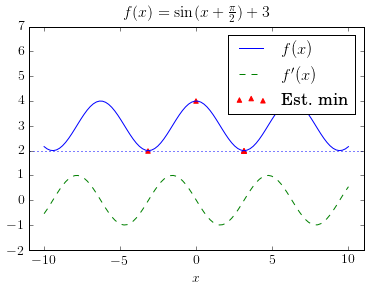
\includegraphics[width=\textwidth]{exercise1d.png}
% 		\caption{A sinusoid and it's derivative, together with the estimated minima}
% 		\label{fig:2var}
% 	\end{subfigure}
% 	\begin{subtable}[b]{0.6\textwidth}
% 	\centering
% 	\begin{tabular}[b]{ccccc}
% 		Guess & Step & Thresh & Iterations & Minimum \\\hline
% 		5 & 0.5 & 0.01 & 9 & ($\pi$, 2) \\\hline
% 		-5 & 0.5 & 0.01 & 9 & ($-\pi$, 2)  \\\hline
% 		0 & 0.5 & 0.01 & 1 & (0, 4) \\\hline
% 		0.5 & 0.5 & 0.01 & 12 & ($\pi$, 2) \\\hline
% 		0.2 & 0.5 & 0.01 & 14 & ($\pi$, 2) \\\hline
% 		0.7 & 0.5 & 0.01 & 11 & ($\pi$, 2) \\\hline
% 	\end{tabular}
% 	\vspace{10mm}
% 	\caption{Parameters and results of gradient descent}
% 	\label{tbl:nomin}
% 	\end{subtable}
% 	}\\
% 	\caption{Using gradient descent on a function with many local minima}
% \end{figure}

% \begin{figure}[!ht]
% \centering
% 	\makebox[\linewidth][c]{%}min}
% \begin{subfigure}[ht]{0.4\textwidth}
% 		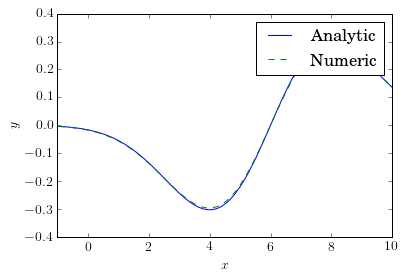
\includegraphics[width=\textwidth]{exercise1e.png}
% 		\label{fig:cdgaus}
% 		\caption{}
% 	\end{subfigure}
% 	\begin{subfigure}[ht]{0.4\textwidth}
% 		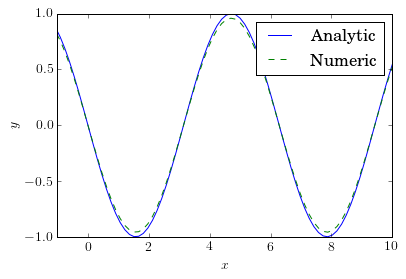
\includegraphics[width=\textwidth]{exercise1f.png}
% 		\label{fig:cdsin}
% 		\caption{}
% 	\end{subfigure}
% 	\begin{subtable}[ht]{0.4\textwidth}
% 	\centering
% 	\begin{tabular}[ht]{ccccc}
% 		(x, y) & Analytic $\nabla f$ & Numeric\\\hline
% 		(-2, -2) & (0, -4) & (0, -4) \\\hline
% 		(-2, -1) & (0, -2) & (0, -2) \\\hline
% 		(-2, 0) & (0, 0) & (0, 0) \\\hline
% 		(-2, 1) & (0, 2) & (0, 2) \\\hline
% 		(-2, 2) & (0, 4) & (0, 4) \\\hline
% 	\end{tabular}
% 	\vspace{5mm}
% 	\label{tbl:2varcd}
% 	\caption{}
% 	\end{subtable}
% 	}\\
% 	\label{fig:centraldiff}
% 	\caption{The step size for calculating the central difference was $1$. (a) The analytic and numeric approximations of Figure \ref{fig:gaus}. (b) The analytic and numeric approximations of Figure \ref{fig:nomin}.  (c) The analytic and numeric approximations of Figure \ref{fig:2var}.}
% \end{figure}

% The gradient of a function can either be specified analytically or numerically approximated with central differences using $\delta_{h}[f](x) = f(x + 0.5h) - f(x - 0.5h)$. From a numerical standpoint, using either the analytical or numerical approximation to the gradient is approximately equivalent, given the correct choice of step size (see Figure 4).


% Software packages like SciPy implement a different algorithm for estimating minima. Table 1 gives a comparison of the number of iterations of the algorithm needed to find a solution. In general, the \textsc{bfgs} optimizer in SciPy performs better than the simple gradient descent algorithm presented here. Both algorithms came up to the same solution within a few significant digits.

The implemented gradient descent procedure was tested on three functions: 
\begin{enumerate}[(a)]
	\item A convex function: $f(x) = -Gaussian(6, 4)$ (an upside-down Gaussian with mean $6$ and variance $4$), who's minimum value is at $(6, -1)$. 
	\item A scalar convex function of two variables: $f(x, y) = (x + 2)^2 + y^2$, who's minimum value is at $(-2, 0)$.
	\item A non-convex function: $f(x) = \sin(x + \frac{\pi}{2})$, who has multiple minima at $(n \pi, -1)$ for all values of $n$.
\end{enumerate}

Figure \ref{fig:1-2-ab} shows the result of calculating the gradient descent on functions (a) and (b) written above. The dots are the calculated minima from gradient descent calculated at multiple step sizes, initial guesses, and thresholds. For convex functions with one minimum, the threshold is the biggest indicator of how many steps the procedure takes to converge. The threshold also determines how close the result is to the real minimum - the smaller the threshold, the closer the result is to the real minimum. Because there is one global minimum, the initial guess does not affect the end result of the function or significantly change the number of iterations required to converge.

\begin{figure}[!ht]
	\centering
	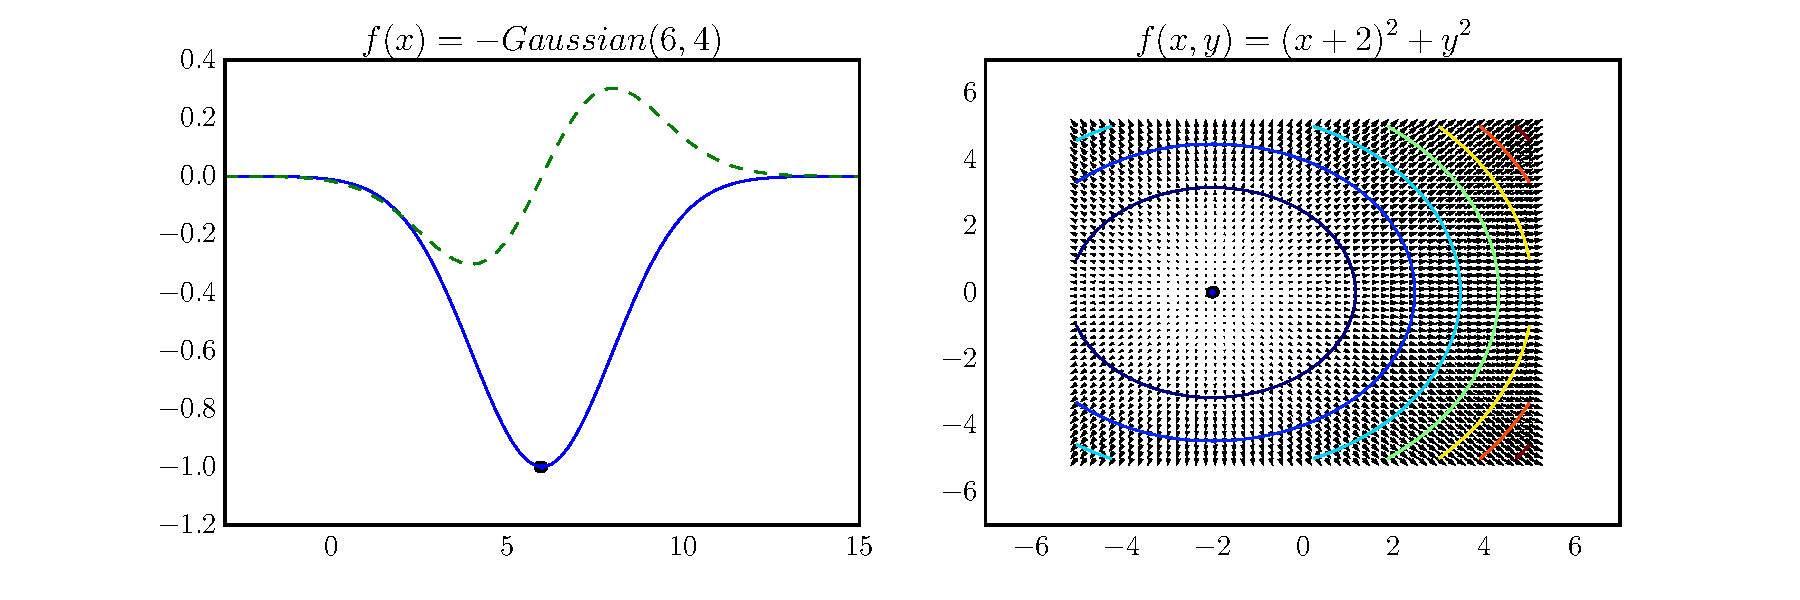
\includegraphics[width=.66\textwidth]{exercise1-2-ab.pdf}
	\caption{(a) Convex function with known minimum value and it's analytical derivative. The dots are the calculated minima according to gradient descent. (b) Contour plot of the gradient of a scalar function with vector-valued arguments. The dots are the calculated minima according to gradient descent.}
	\label{fig:1-2-ab}
\end{figure}

Figure \ref{fig:1-2-c} shows the result of using gradient descent on function (c) with different parameters. The sequence of dots in each case represents the guesses that gradient descent takes to be the minimum. In general, the choice of starting point affects which local minimum gradient descent will find. If the starting point chosen is a local maximum, the procedure will not step towards a minimum because the gradient is zero at the maximum. If the step size is large, the procedure will overshoot the minimum and zig-zag back to the desired minimum, taking a large number of iterations to converge. 

\begin{figure}[!ht]
	\centering
	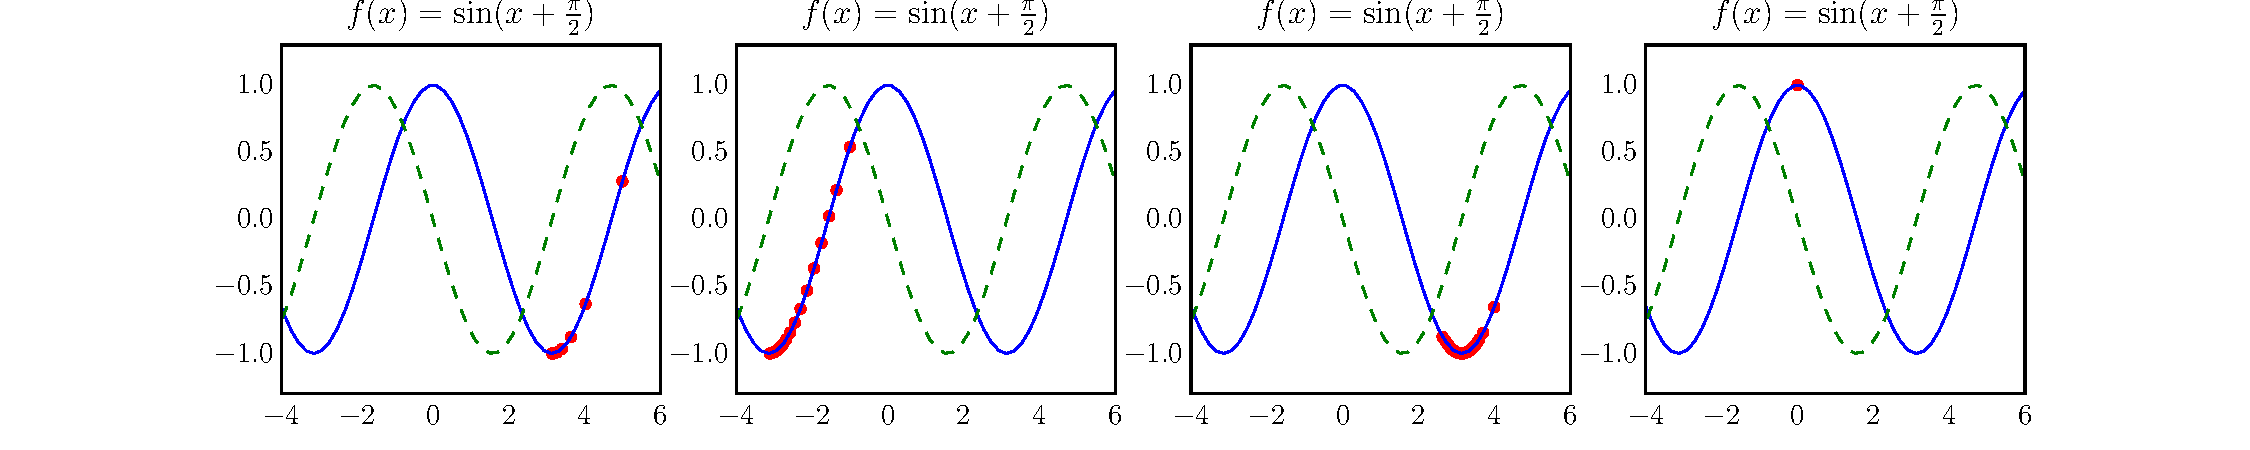
\includegraphics[width=\textwidth]{exercise1-2-c.pdf}
	\caption{The solid line is the function, the dashed line is its analytical derivative, and the series of dots is the series of minimum guesses from gradient descent. (a) Initial guess: 5, step: 0.5, threshold: 0.1 converges in 9 iterations. (b) Initial guess: -2, step: 0.2, threshold: 0.1 converges in 20 iterations. (c) Initial guess: 4, step: 2, threshold: 0.1 converges in 59992 iterations. (d) Initial guess: 0, step: 0.5, threshold: 0.1 converges in 1 iteration, but does not converge to a minimum. }
	\label{fig:1-2-c}
\end{figure}

Approximating a function's gradient using central differences is very accurate if using an $h$ of $1$. Figure \ref{fig:1-3-a} shows graphs of either the gradient function or gradient vector field for the three functions tested above. It is hard to tell the difference between the analytical and numerical functions, so using central differences to numerically estimate the gradient is effective.

\begin{figure}[!ht]
	\centering
	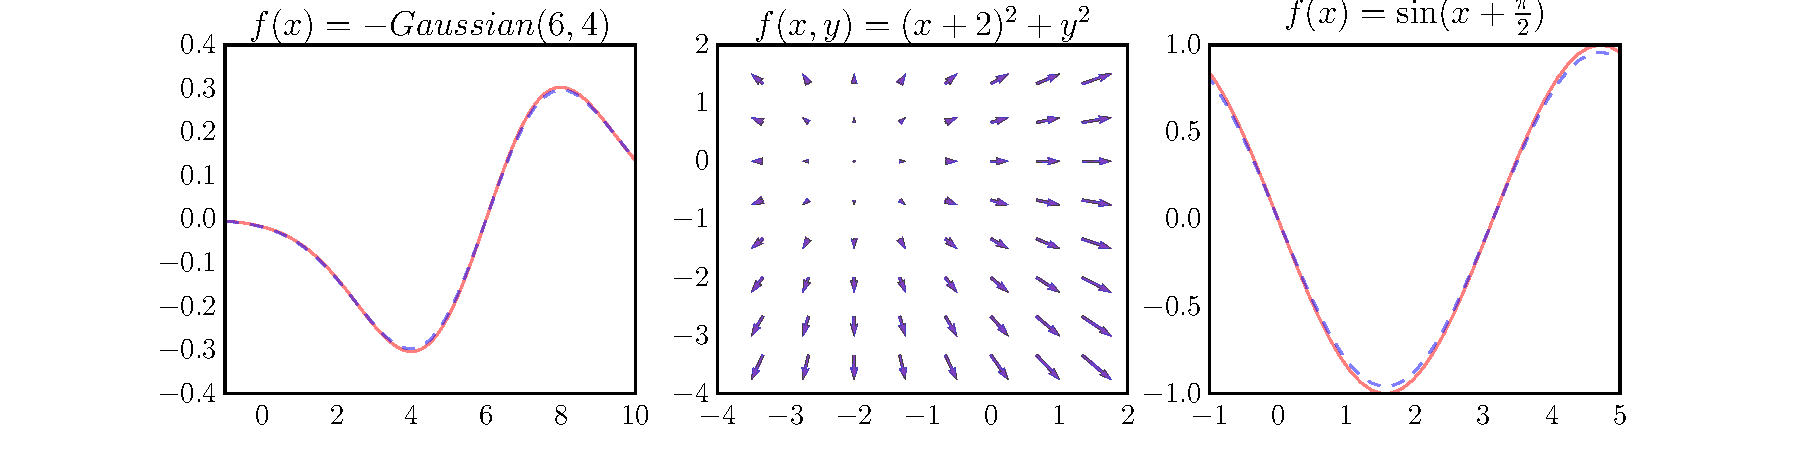
\includegraphics[width=\textwidth]{exercise1-3-a.pdf}
	\caption{The analytical and numerical gradients for the functions (a) upside-down Gaussian, (b) $f(x, y)= (x + 2)^2 + y^2$, and (c) $f(x) = \sin(x + \frac{\pi}{2})$. The solid red line is the analytical gradient and the dashed blue line is the numerical gradient.}
	\label{fig:1-3-a}
\end{figure}

The \textsc{BFGS} optimizer in SciPy uses a more sophisticated method for estimating minima, so in general, the number of function evaluations needed before convergence is smaller. Table \ref{tbl:1-4-a} shows a comparison of the gradient descent and \textsc{BFGS} optimizer, where in all cases the step size was $0.2$ and the threshold was $0.01$.

\begin{table}[!ht]
\centering
\makebox[\textwidth][c]{
\begin{tabular}[ht]{ccccc}
Function & Initial Guess & Algorithm & Evaluations & Min at\\\hline
\multirow{2}{*}{$f(x) = -$Gaussian$(6, 4)$} & \multirow{2}{*}{$x = 5$} & GD & 34 & $x = 5.81$ \\
 & & \textsc{BFGS} & 6 & $x = 6.00$ \\\hline
\multirow{2}{*}{$f(x, y) = (x + 2)^2 + y^2$} & \multirow{2}{*}{$(x, y) = (5, 5)$} & GD & 13 & $(x, y) = (-2, 0)$\\
 & & \textsc{BFGS} & 4 & $(x, y) = (-2, 0)$ \\\hline
\multirow{2}{*}{$f(x) = \sin(x + \frac{\pi}{2})$} & \multirow{2}{*}{$x = 5$} &  GD & 20 & $x = 3.15$ \\
 & &  \textsc{BFGS} & 6 & $x = 3.14$ \\
\end{tabular}
}
\caption{Steps to convergence given a similar set of parameters. GD is gradient descent, \textsc{BFGS} is from SciPy. For gradient descent, all step sizes were $0.5$ and thresholds were $0.01$.}
\label{tbl:1-4-a}
\end{table}

% \newpage
\section{Exercise 2}

\begin{figure}[!ht]
	\centering
	\makebox[\textwidth][c]{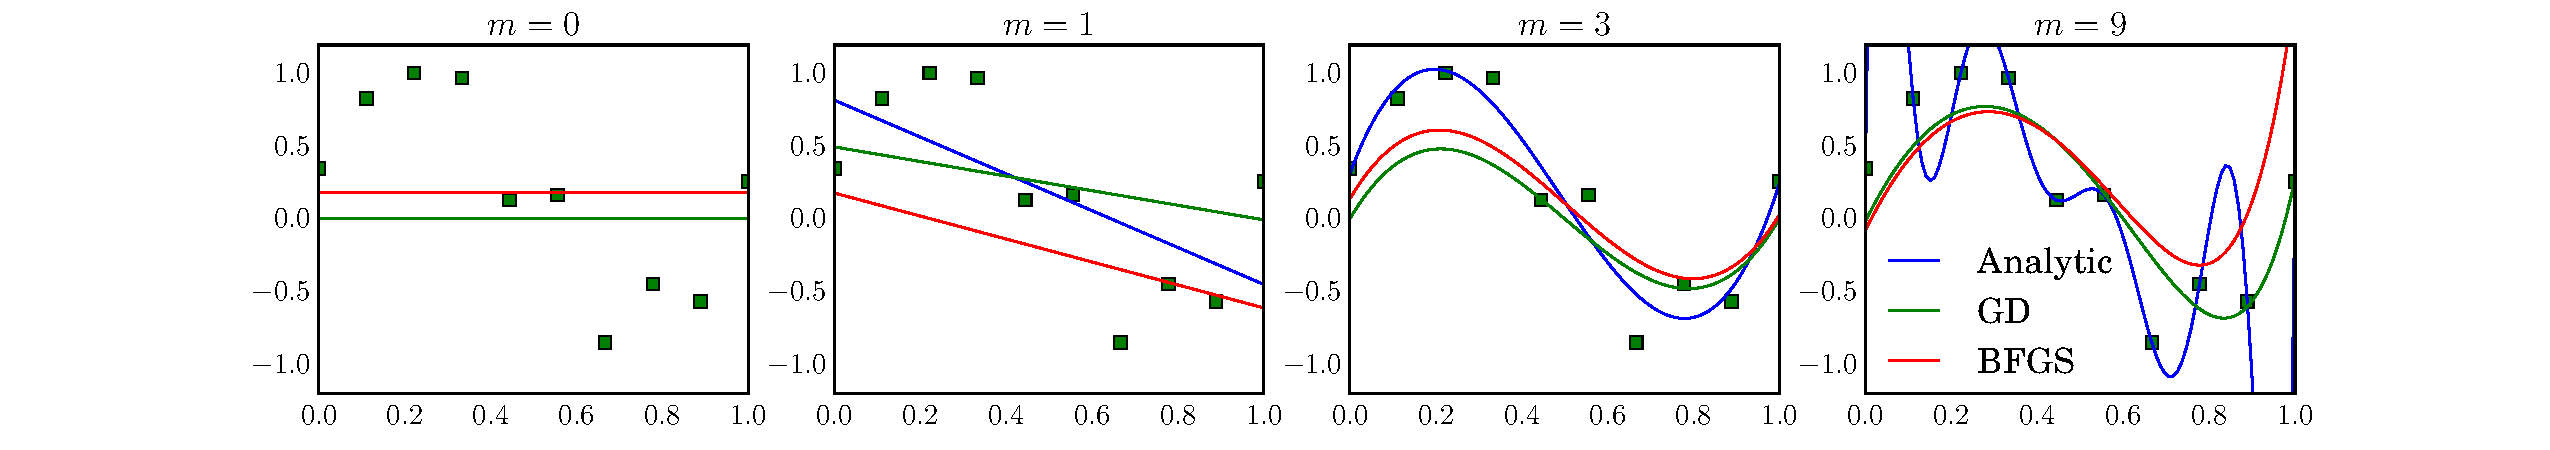
\includegraphics[width=1.25\textwidth]{exercise2-1.pdf}}
	\caption{Plots replicating Figure 1.4 in Bishop for different values of $M$ using different methods. The blue is generated with the analytical solution of the SSE, the green with the gradient descent method on the SSE, and the red using Python's \textsc{BFGS} optimizer.}
	\label{fig:2-1}
\end{figure}

\begin{figure}[!ht]
\centering
\makebox[\textwidth][c]{
\begin{subtable}[!ht]{0.5\textwidth}
\centering
\scalebox{0.8}{
\begin{tabular}{l|rrrr}
	& $M = 0$ & $M = 1$ & $M = 6$ & $M = 9$ \\\hline
	$\hat{w}_0$ & $0.186$ & $0.820$ & $0.353$ & $0.349$ \\
	$\hat{w}_1$ & & $-1.268$ & $2.619$ & $232.411$\\
	$\hat{w}_2$ & & & $32.096$ & $-5322.833$\\
	$\hat{w}_3$ & & & $-206.273$ & $48577.404$\\
	$\hat{w}_4$ & & & $399.001$ & $-231682.150$\\
	$\hat{w}_5$ & & & $-332.709$ & $640159.305$\\
	$\hat{w}_6$ & & & $105.163$ & $-1061992.54$\\
	$\hat{w}_7$ & & & & $1042586.68$ \\
	$\hat{w}_8$ & & & & $-557781.754$\\
	$\hat{w}_9$ & & & & $125223.393$\\
\end{tabular}
}
\end{subtable}
\hspace{3mm}
\begin{subtable}[!ht]{0.5\textwidth}
\centering
\scalebox{0.8}{
\begin{tabular}{l|rrrr}
	& $M = 0$ & $M = 1$ & $M = 6$ & $M = 9$ \\\hline
	$\hat{w}_0$ & $0.003$ & $0.499$ & $0.623$ & $-0.014$ \\
	$\hat{w}_1$ & & $-0.502$ & $5.577$ & $6.018$ \\
	$\hat{w}_2$ & & & $-14.465$ & $-12.820$ \\
	$\hat{w}_3$ & & & $5.502$ & $6.294$ \\
	$\hat{w}_4$ & & & $0.475$ & $-5.629$ \\
	$\hat{w}_5$ & & & $0.453$ & $4.425$ \\
	$\hat{w}_6$ & & & $0.435$ & $0.464$ \\
	$\hat{w}_7$ & & & & $0.493$ \\
	$\hat{w}_8$ & & & & $0.516$ \\
	$\hat{w}_9$ & & & & $0.533$ \\
\end{tabular}}
\end{subtable}
\begin{subtable}[!ht]{0.5\textwidth}
\centering
\scalebox{0.8}{
\begin{tabular}{l|rrrr}
	& $M = 0$ & $M = 1$ & $M = 6$ & $M = 9$ \\\hline
	$\hat{w}_0$ & $0.186$& $0.181$ & $0.133$ & $-0.077$ \\
	$\hat{w}_1$ & & $-0.791$ & $4.974$ & $6.080$ \\
	$\hat{w}_2$ & & & $-0.150$ & $-12.746$ \\
	$\hat{w}_3$ & & & $4.964$ & $6.398$ \\
	$\hat{w}_4$ & & & $-0.027$ & $-5.494$ \\
	$\hat{w}_5$ & & & $-0.020$ & $4.586$ \\
	$\hat{w}_6$ & & & $-0.013$ & $0.646$ \\
	$\hat{w}_7$ & & & & $0.692$ \\
	$\hat{w}_8$ & & & & $0.729$ \\
	$\hat{w}_9$ & & & & $0.758$ \\
\end{tabular}}
\end{subtable}
}
\caption{Table 1.1 from Bishop replicated using (a)analytical solutions, (b) gradient descent, and (c) the Scipy \textsc{BFGS} optimizer}
\end{figure}

\section{Exercise 3}

This is a test. 

\section{Exercise 4}

This is a test. 

\end{document}